\documentclass[11pt,table]{article}
\usepackage{jeffe,handout}
\usepackage{fancyvrb}
\usepackage{tikz}
\usepackage{pgfkeys}
\usepackage{array,relsize}
%\usepackage[shortlabels,inline]{enumitem}
\usepackage[shortlabels,inline]{enumitem}
\newcolumntype{E}{>{\centering\arraybackslash}p{9mm}}
\newcolumntype{P}{>{\centering\arraybackslash}p{5mm}}
\newcolumntype{Q}{>{\centering\arraybackslash}p{2mm}}
\newcommand{\elide}[1]{}

\usepackage{multicol}
\newcommand{\marksamt}[1]{\textbf{[#1~marks]}}
\newcommand{\markamt}[1]{\textbf{[#1~mark]}}
\newcommand{\fillinMC}[1]{\fillinMCmath{\mbox{#1}}}
\newcommand{\fillinMCmath}[1]{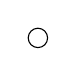
\begin{tikzpicture}\draw circle [radius=0.35em];\end{tikzpicture}\ #1}

\newcommand{\filledMC}[1]{\filledMCmath{\mbox{#1}}}
\newcommand{\filledMCmath}[1]{
\begin{tikzpicture}\draw[fill=black] circle [radius=0.35em];\end{tikzpicture}\ #1}

\newcommand{\fillinMCAll}[1]{\fillinMCAllmath{\mbox{#1}}}
\newcommand{\fillinMCAllmath}[1]{\begin{tikzpicture}\draw (0,0) rectangle (1em,1em);\end{tikzpicture}\ #1}
\newcommand{\fillinblank}[1]{\fillinblankmath{\mbox{#1}}}
\newcommand{\fillinblankmath}[1]{\begingroup\setlength{\fboxsep}{1em}\setlength{\fboxrule}{2pt}\fbox{\LARGE\phantom{#1}}\endgroup}

\newcommand{\filledblank}[1]{\filledblankmath{#1}}
\newcommand{\filledblankmath}[1]{\begingroup\setlength{\fboxsep}{1em}\setlength{\fboxrule}{2pt}\fbox{\LARGE{#1}}\endgroup}

\newcommand{\filledSblank}[1]{\filledSblankmath{#1}}
\newcommand{\filledSblankmath}[1]{\begingroup\setlength{\fboxsep}{1em}\setlength{\fboxrule}{2pt}\fbox{#1}\endgroup}

\newcommand{\blank}{\rule{3mm}{0.1mm}}
\newcommand{\blankk}{\rule{2cm}{0.1mm}}
\newcommand{\shade}{\cellcolor[gray]{0.8}}

%\def\rmdefault{bch} % Use Charter for main text font.
\usepackage{tikz}
\usepackage{tikz-qtree}




% definitions for formatting code blocks
\usepackage{listings}
%\usepackage{color}
\definecolor{dkgreen}{rgb}{0,0.6,0}
\definecolor{gray}{rgb}{0.5,0.5,0.5}
\definecolor{mauve}{rgb}{0.58,0,0.82}

\lstset{frame=tb,
  language=C++,
  aboveskip=3mm,
  belowskip=3mm,
  showstringspaces=false,
  columns=flexible,
  basicstyle={\small\ttfamily},
  numbers=left,
  numberstyle=\tiny\color{gray},
  keywordstyle=\color{blue},
  commentstyle=\color{dkgreen},
  stringstyle=\color{mauve},
  breaklines=true,
  breakatwhitespace=true,
  tabsize=3
}

% end definitions for formatting code blocks

\def\BOX#1{\fbox{\vbox to #1{\vss\hbox to #1{\hss}}}}
\def\Bigbox{\BOX{0.25in}}
\def\Bigbox{\raisebox{-0.5ex}[0.25in][0pt]{\BOX{0.25in}}}
\def\problem#1{\def\problemheading{#1}\clearpage\item{\bf #1.}}

\hidesolutions

\renewcommand{\arraystretch}{2}

% =========================================================
\begin{document}

\headers{CPSC 221}{ }{Winter 1, 2019}

\begin{center}
    \LARGE
    \textbf{Assignment 2}
    \\[1ex]
    \Large Due 23:59, Friday, October 4, 2019 \\
\end{center}

\begin{table}[h]
    \centering
    \renewcommand{\arraystretch}{1.5}
    \begin{tabular}{ll}
%        \textbf{Name}: & \\
%        \textbf{Student ID}: & \\
        \textbf{CS ID 1}: & \textbf{d6a2b}\\
        \textbf{CS ID 2}: & \textbf{z0n1b}\\
    \end{tabular}
\end{table}

\textbf{Instructions:}
\begin{enumerate}
\item Do not change the problem statements we are giving you. Simply add your solutions by editing this latex document. 
\item Take as much space as you need for each problem. You'll tell us where your solutions are when you submit your paper to gradescope. 
\item Export the completed assignment as a PDF file for upload to gradescope.
\item On gradescope, upload only \textbf{one} copy per partnership. (Instructions for uploading to gradescope will be posted on the HW2 page of the course website.)
\end{enumerate}

\newpage
\begin{enumerate}

\newcommand{\I}{\ensuremath{\mathit{I}}}
\renewcommand{\O}{\ensuremath{\mathit{O}}}
\renewcommand{\E}{\ensuremath{\mathit{E}}}
\newcommand{\D}{\ensuremath{\mathit{D}}}

\problem{Dead Heads (25 points)}

In some cases, it's easier to handle the special case of deleting the head of a linked-list or inserting a new node in front of the head of a linked-list by using a \emph{dead head} (sometimes called a \emph{dummy head}, or \emph{sentinel}).
The dead head is always the first node in the linked-list but it contains no data. (You can think of it as an empty node!)
Its \texttt{next} pointer points to the ``real'' head of the linked-list, that is the first node in the linked-list that contains valid data.
So an empty linked-list is represented by a dead head whose \texttt{next} pointer is \texttt{NULL}.  
The user specifies the linked-list by using a pointer to the list's dead head.
For this problem, you will fix some implementations that use dead-headed linked-lists as a private member representation of a \texttt{List} class.

Here is the \texttt{List} class definition that we will examine and expand:
\begin{verbatim}
class List{
  public: 
    void addAt(int pos, int elt);
    void delAll(int x);
  private:
    struct Node{
      int data;
      Node * next;
      Node(int elt = 0,Node * p = NULL):data(elt),next(p){}
    };
    Node * head;
    Node * walk(Node * curr, int k);
    void delNode(Node * p);
};

List::Node * List::walk(List::Node * curr, int k){
  // walks curr forward k steps
  if (k<=0 || curr == NULL)
    return curr;
  else return walk(curr->next, k-1);
}

\end{verbatim}

\begin{enumerate}
\item (2 points) Write the no-argument constructor for the above \texttt{List} class if the class is designed so that the empty list is represented by a single dead head node.

\begin{Verbatim}[frame=single,framerule=2pt]
List::List(){
  head = new Node();
}
\end{Verbatim}

\item (2 points)
Suppose that you have designed class \texttt{List} to contain a linked list implemented \emph{without} a dead head. (We will refer to this implementation as the ``Live Head'' implementation, which is not an official term!) Write member function \texttt{addAt(int pos, int e)} which creates a new node at position \texttt{pos} whose data is \texttt{e}. Note that in this case we consider the first data element of the list to be position 0, and that in an empty list, \texttt{head == NULL}. Please use the given \texttt{walk} function to advance
a pointer along the list.

\begin{Verbatim}[frame=single,framerule=2pt]
void List::addAt(int pos, int elt){
  //we may assume that pos is valid, only range is [0,size]
  //where pos=0 is add to beginning, before everything
  //and pos=size is add to end, after everything
  //piazza 693
  Node *offset = new Node;
  offset->next = head;
  Node *toAdd = walk(offset, pos);
  Node *newnode = new Node;
  newnode->data = elt;
  newnode->next = toAdd->next;
  toAdd->next = newnode;
  if (pos == 0) {
    head = newnode;
  }
  delete offset;
}
\end{Verbatim}

\item (2 points)
Rewrite the \texttt{addAt} member function for a list designed to use a dead head at the front of the list. Note that in this case we consider the first data element of the list to be position 0.
You may assume that member variable \texttt{head} is not \texttt{NULL}, even if the list is empty.
 
\begin{Verbatim}[frame=single,framerule=2pt]
void List::addAt(int pos, int elt){
  //we may assume that pos is valid, only range is [0,size]
  //where 0 is add before everything but after deadhead
  //and size is add after everything
  //piazza 693
  Node *toAdd = walk(head, pos);
  Node *newnode = new Node;
  newnode->data = elt;
  newnode->next = toAdd->next;
  toAdd->next = newnode;
}
\end{Verbatim}

\item (2 points) Research the meaning of the term \emph{cyclomatic complexity}, and use your understanding to answer the following questions.\\

Which implementation of \texttt{addAt} has lower cyclomatic complexity?\\
\begin{enumerate*}
% use \filledMC{} for your choice.
\item[\checkmark] Dead Head\hspace{0.5cm}
\item[\fillinMC{}] Live Head\hspace{0.5cm}
\end{enumerate*}\\

Given their relative cyclomatic complexities, we expect the number of test cases for the dead head implementation to be \begin{enumerate*}
% use \filledMC{} for your choice.
\item[\fillinMC{}] greater than\hspace{0.5cm}
\item[\checkmark] less than\hspace{0.5cm}
\item[\fillinMC{}] equal to\hspace{0.5cm}
\end{enumerate*} the number we would need for the live head implementation of \texttt{addAt}.

\item (4 points) The following \texttt{List} class member function is intended to delete all nodes with data equal to $x$ from a dead-headed linked-list whose last node has a \texttt{NULL} next pointer.
It doesn't always work.
Two lines of code need to be corrected.
Write the correct lines in the boxes next to the two lines that are incorrect.

\bgroup
\renewcommand{\arraystretch}{1.5}
\begin{tabular}{l|p{7.3cm}|}
\cline{2-2}
\verb|void List::delAll(int x){|&\\
\cline{2-2}
\verb|  a = head;|& \(\)\\
\cline{2-2}
\verb|  while ( a->next != NULL ) {|&\\
\cline{2-2}
\verb|    if ( a->next->data == x ) {|&\\
\cline{2-2}
\verb|      Node *t=a;|& \(Node *t = a->next;\)\\
\cline{2-2}
\verb|      a->next = a->next->next;|&\\
\cline{2-2}
\verb|      delete t;|&\\
\cline{2-2}
\verb|    }|&\\
\cline{2-2}
\verb|    a = a->next;|&\(else \{a = a->next;\} \)\\
\cline{2-2}
\verb|  }|&\\
\cline{2-2}
\verb|}|&\\
\cline{2-2}
\end{tabular}
\egroup

\end{enumerate}

In this part of the problem, we will explore an algorithm for removing a node from a singly linked list containing $n$ nodes \emph{given a pointer to the node we wish to remove}. 
\begin{enumerate}[resume]

\item (3 points) This removal task would be simple if we had a 
pointer to the node \emph{before} the one we wish to 
remove. We can be sure there \emph{is} a node before the one we wish to remove if we implement the list with a dead head. Complete the code below to implement the \texttt{List} class member function that removes node \texttt{p} from the list whose \texttt{head} is a dead head, using the comments to guide your algorithm.
You may assume that \texttt{p} is a valid data element from the linked list.

\begin{Verbatim}[frame=single,framerule=2pt]
void List::delNode(Node *p){
  Node * t = head;
  
  /* advance t until it's in a useful place */
  //no need for t->next == NULL guard if we know p exist in list
  while (t->next != p) {
    t = t->next;
  }
  
  /* adjust pointers to remove appropriate node */
  t->next = t->next->next;
  
  /* free memory associated with p */
  delete p;
  p = NULL;
}
\end{Verbatim}

\item (1 point) The worst case running time of \texttt{delNode} is \begin{enumerate*}
% use \filledMC{} for your choice.
\item[\fillinMC{}]
$\Theta(1)$\hspace*{0.5cm}
\item[\fillinMC{}]
$\Theta(\log n)$\hspace*{0.5cm}
\item[\checkmark]
$\Theta(n)$
\end{enumerate*}

\item (4 points)
If we are clever, we can solve the problem of removing a node, given a pointer to it, \emph{without} iterating over the list. To solve this problem, consider the pointer you are given, and ask yourself which node \emph{would} be easy to remove. Is there a way to remove that
node, while at the same time preserving its data? 
The following function is intended to effectively delete the node pointed to by \texttt{p} from a linked-list with a dead head.
Complete the code below so that it takes constant time to do this operation.
You may assume that \texttt{p} points to a valid data node (not the dead head). 

\begin{Verbatim}[frame=single,framerule=2pt]
void List::delNode(Node *p){
  //"delete the node pointed to by p" = delete p->next
  /* set up a pointer to a node that would be easy to remove */
  Node * t = p->next;

  /* preserve the data contained in that node */
  p->data = p->next->data;

  /* fix pointers */
  p->next = p->next->next;
  
  /* free appropriate memory */
  delete t;
}
\end{Verbatim}

\item (2 points) You probably noticed that this algorithm fails if the input parameter \texttt{p} points to a particular node. 
\begin{enumerate}
    \item The code fails if \texttt{p} is a pointer to what node?

\begin{Verbatim}[frame=single,framerule=2pt]
The last node, because p->next = NULL, 
and p->next->data is undefined behaviour.
\end{Verbatim}


    \item Describe how you would change the design of the linked list so that the algorithm above would work for any valid \texttt{p} (where ``valid'' means that it points to a node with data).
    
\begin{Verbatim}[frame=single,framerule=2pt]
Since there's only one edge case, adding a guard saying 
if(p->next == NULL) { 
  //walk the list to get node before p
  //set that node's next to NULL, and free p
} else { 
  //do the same thing
} 
is enough.
\end{Verbatim}
\end{enumerate}
\item (3 points)
This mechanism for removing a node from a list is commonly referred to as a constant time ``hack'' because it exhibits some important disadvantages. Choose the applicable disadvantages from the list below.\\

\begin{tabular}{cl}
% use \filledMC{} for your choices.
\checkmark &  If \texttt{p->data} is a large object, the execution of the function may be very slow. \\
\fillinMC{} &  The compiler cannot optimize the amount of memory needed by the \texttt{Node}.\\
\checkmark &  In order to work, the assignment operator must be implemented for data's type. \\
\fillinMC{} &  There could be be a memory leak. \\
\fillinMC{} &  The implementation requires a dead head. \\
\fillinMC{} &  The constant time code will only work on lists with more than one data element. \\
\checkmark &  An iterator over the list may be invalidated. \\
\checkmark &  This code may result in a 
segmentation fault due to dereferencing a \texttt{NULL} pointer. \\
\end{tabular}
\end{enumerate}

\problem{Structured Sorting (22 points)}

We want to sort a sequence of numbers using a stack.
We imagine the numbers arrive at the stack in their input order.  For example, if the input is 5,1,4,2,3 then 5 arrives first and 3 arrives last.
When a number arrives, we must push it onto the stack and then we can perform any number of pop operations (including none).
Each pop operation not only pops the top number off of the stack it also outputs the number.
Pops on an empty stack are invalid.
We want the sequence of numbers that are output to be the original input sequence in non-decreasing order.

For example, the following operation sequence sorts 5,1,4,2,3: \I\I\O\I\I\O\I\O\O\O{} where \I{} means ``push In'' and \O{} means ``pop Out''.

\begin{enumerate}

\item (2 points)
Some operation sequences attempt to pop from an empty stack
or end before the stack is empty.  These are called \emph{invalid}
sequences.
Describe two simple conditions that together ensure that an operation sequence is valid.

% Replace with \filledSblank{ your answer }    
    \filledSblank{At any point of the sequence you cannot have more Os before Is}\\
    
    \filledSblank{The sequence must have the same number of Is and Os if you want to end }

\item (2 points)
What input sequence using the numbers 1,2,3 cannot be sorted in this way; meaning no sequence of operations will sort the given input.

% Replace with \filledblank{ your answer }
\filledSblank{2,3,1}

\item (8 points)
Prove that it is impossible to sort an input sequence in which the number $b$ is before the number $c$ which is before the number $a$ and $a < b < c$.

\hrulefill
\begin{Verbatim}
Input: b,c,a
Output: a,b,c

Steps:
1. With output of a,b,c, a has to be pop first. To
pop a, we have to push a. With input of b,c,a, we 
have to push b,c first. 
2. We can't pop b,c while pushing because a is 
supposed to come first in output ordering, so the 
order on the stack when the stack is full is 
b,c,a. 
3. Once we popped a, the top of stack is c, since 
b was pushed first, so c must be the next to pop.

Since c comes after b, our output is not sorted. 
If we decide to pop b before c, we'll contradict 
step 2's logic and a is not in order. Therefore, 
this sequence can't be sorted with just a stack.
\end{Verbatim}
\vspace{2.5in}
\end{enumerate}

Suppose we add the choice of a queue to our sorting algorithm.
Now we can use the operations \I, \O, \E, and \D{}, where \I{} and \O{} push and pop the stack, while \E{} and \D{} enqueue and dequeue the queue (dequeue also outputs the number that is dequeued).
For example,
we can sort 5,1,4,2,3 using:
\I\E\I\E\E\D\D\D\O\O.

\begin{enumerate}[resume]

\item (2 points)
What input sequence using the numbers 1,2,3,4 is sorted by the sequence of operations \E\I\E\I\O\O\D\D?

% replace with \filledblank{ your answer }
\filledSblank{3,2,4,1}

\item (4 points)
Is it possible to sort all input sequences using such a stack and queue?  If yes then explain how.
If no, give a permutation that cannot be output.

\hrulefill
\begin{Verbatim}
A sample sequence:
4,2,5,1,3

\end{Verbatim}
\vspace{0.2in}

\item (4 points)
Suppose we add two new operations.\\
$S$ : pop a number from the stack (without output) and enqueue it into the queue; and\\
$Q$ : dequeue a number from the queue (without output) and push it onto the stack.\\
Is it possible to sort all input sequences
using the operations \I, \O, \E, \D, $S$, and $Q$?  If yes then
explain how.  If no, give a permutation that cannot be output.

\hrulefill
\begin{Verbatim}
Definition:
X: input array, with integers from [m,n] unsorted
Y: output array, with integers from [m,n] sorted
k: arbitrary integer from X
j: the largest number in X that is still smaller than k
i: current position while iterating through X, with max i being X.size-1
f: smallest previously sorted integer, ie top of stack (this definition used in 
inductive step)
g: largest previously sorted integer, ir back of queue (this definition used in 
inductive step)

We have an array input X, and we want output array Y. We know from part e that if 
we have a sorted queue from k (front) to n (back), and a sorted stack of m (top) 
to j (bottom), we can pop all integers from m to j, and dequeue all integers from 
k to n, to have sorted output array. Therefore, this is an inductive proof of how 
we can use operations to keep queue and stack sorted when receiving new integer 
from input array.

Base case: Since we referenced 4 variables in our introduction, we can say that 
the base case input has 4 integers. Suppose they are a,b,c,d for simplicity, where 
a<b<c<d. There are 24 possible input arrangements, and therefore 24 possible ways 
to create sorted queue {c,d} and stack {a,b}, written here using the previously 
defined shorthands.

{a,b,c,d}: EIEEQ
{a,b,d,c}: EIIESQ
{a,c,b,d}: EEIQE
{a,c,d,b}: EEEIQ
{a,d,b,c}: EEIEQQS
{a,d,c,b}: EEEIQQS
{b,a,c,d}: IIEE
{b,a,d,c}: IIEEQS
{b,c,a,d}: IEIE
{b,c,d,a}: IEEI
{b,d,a,c}: IEIEQS
{b,d,c,a}: IEEIQS
{c,a,b,d}: EEIEQSQQS
{c,a,d,b}: EEEIQSQQS
{c,b,a,d}: EIIE
{c,b,d,a}: EIEI
{c,d,a,b}: EEEIQSQSQ
{c,d,b,a}: EEII 
{d,a,b,c}: EEEEQSQSQQSQSQ
{d,a,c,b}: EEEIQSQ
{d,b,a,c}: EIIEQS
{d,b,c,a}: EIEIQS
{d,c,a,b}: EEEIQSQSQQS
{d,c,b,a}: EEIIQS

As a sidenote, there also are base cases where X's size is 0,1,2,3 which are not 
relevant to the inductive step, but still key to the proof as a whole. Since it is 
a small amount of cases, we can exhaustively prove that we can obtain Y. As 
previously define, a<b<c. For step, we can't divide X into a neat queue and 
stack pair, but we can just show directly that we can achieve Y.
{}: empty list is sorted by definition
{a}: list with one member is sorted definition, so just IO
{a,b}: ED
{b,a}: IO
{a,b,c}: EEEDDD
{a,c,b}: EEIDOD
{b,a,c}: IIEOOD
{b,c,a}: EEIODD
{c,a,b}: IEIDOO
{c,b,a}: IIIOOO

Inductive hypothesis: For all past numbers in input array from X[0] to X[i], we 
assume that they are sorted such that all integers are separated into two groups 
using an arbitrary k selected from X[0] to X[i], with integers from m to j is 
sorted in stack, and integers from k to n is sorted in queue.

Inductive step: For X[i+1], it has to either be (1)[m,f], (2) (f,j] , (3) [k,g), 
(4) [g,n]. We can break inductive step into four cases.

Case 1) 
Since it's the smallest yet, it has to go on top of stack. Simply do I operation 
on X[i+1]. After this, our stack should look like {X[i+1],f...j}, and our queue is
not modified. Inductive hypothesis is restored.

Case 2)
Since it is somewhere in the stack, we can do S operation on stack elements until 
X[i+1] is more the previously popped element (we will call this w) and less than 
or equal to the current top of stack (we will call this v). We can do I operation 
on X[i+1]. At this point, the queue has elements such that {k...n,f...w}. Then we 
can do QS operations (which simply puts front of queue to back of queue) on queue 
elements until w is in front of queue, then we do Q operation on w. After doing Q 
operation on w, the queue should look like {k...n,f...z}, where z is the next 
smallest integer from w. We can iterate QS and Q operations until all of f to z is
moved back to stack. After this, our stack should look like 
{f...z,w,X[i+1],v...j}, and our queue should look like {k...n}. Inductive 
hypothesis is restored.

Case 3)
Since it is somewhere in the queue, we can do QS operation on queue elements until
X[i+1] is more or equal to the previously operated queue element (we will call 
this w) and less than the current front of queue (we will call this v). We can do 
E operation on X[i+1]. At this point, the queue has elements such that 
{v...g,k...w,X[i+1]}. Then, we can keep doing QS operation on queue elements up 
until g. After this, queue should look like {k...w,X[i+1],v...g}, and stack is not
modified. Inductive hypothesis is restored.   

Case 4)
Since it's the largest yet, it has to go to back of queue. Simply do E operation 
on X[i+1]. After this, our queue should look like {k...g,X[i+1]}, and our stack is
not modified. Inductive hypothesis is restored.

Conclusion: We can restore the inductive hypothesis for all 4 cases of X[i+1]. 
Therefore, we can say that the inductive hypothesis is proved and we can conclude 
that is a way to keep queue and stack sorted when receiving new integer from input
array, which means that it is always possible to give output Y by popping all 
integers from m to j from stack, and dequeuing all integers from k to n from queue.

\end{Verbatim}

\vspace{.1in}


\end{enumerate}

\problem{Loop Invariants (18 points)}

\begin{enumerate}
Consider the following code for finding a maximum element in an array:
\begin{verbatim}
// Find a maximum element in the array A.
int findMax( int *A, int n ) {
  return findMaxHelper(A, 0, n);
}

// Return the maximum element in A[left..right-1]
int findMaxHelper(int *A, int left, int right) {
  if( left == right - 1 ) return A[left];
  else {
    int max1 = findMaxHelper(A, left, (right + left) / 2);
    int max2 = findMaxHelper(A, (right + left) / 2, right);
    if max1 > max2 return max1 else return max2;
  }
}
\end{verbatim}
\begin{enumerate}

\item (5 points)
Let $n$ be the length of the array \verb|A| and assume $n \geq  1$.
Use induction to prove that this code correctly returns the maximum element in the array.

{ \setlength{\fboxrule}{2pt}
\fbox{
\begin{minipage}{\linewidth}
\textbf{Claim:}
\texttt{findMaxHelper(A, left, right)} returns the maximum element in
\texttt{A[left..right-1]}.

\begin{proof}
% Remove the next two lines and add your proof here.

Base case: Choose n = 1, for n=1 max1 and max2 findMaxHelper(A, 0, 1) will just return the only element in the array A, and since it's the only element, it is also the largest. \\

Inductive Hypothesis: Assume array with length n $	\leq$ k where k is an arbitrary integer, findMaxHelper(A, 0, k) will return the maximum element in that array.\\ 

Inductive Step: IH must also be true for k+1 to successfully prove. In the recursive function findMaxHelper we can see that max1 will recursive be:\\
findMaxHelper(A, 0, k+1)\\
findMaxHelper(A, 0, (k+1)/2)\\
...\\
findMaxHelper(A, 0, 2)\\
findMaxHelper(A, 0, 1)\\
and since max2 is calculated after max1 it will be:\\
findMaxHelper(A, 1, 2);\\
...\\
findMaxHelper(A, (k+1)/2, k+1);\\

By our inductive hypothesis, since we know findMaxHelper will return the largest value in the array within the given length if length $\leq$ k. we know that\\
int max1 = findMaxHelper(A, 0, (k+1)/2) and \\
int max2 = findMaxHelper(A, (k+1)/2, k+1)\\
will return the max element in the first half (max1) and second half(max2) of the original array of length k+1. (Since both of their length are shorter than k) Afterwards, the subsequent inequality statement will compare max1 and max2 to return the maximum element of the array from 0 to k+1, which proves our inductive hypothesis to be correct.  


\mbox{}\par
\vspace{3in}
\end{proof}
\end{minipage}
}}

\item (5 points)
Let $T(n)$ be the run time of this algorithm.
Express $T(n)$ as a recurrence relation.
Use repeated substitution (ignore floors/ceilings when calculating $n/2$)
to determine a closed-form solution for $T(n)$, i.e., express $T(n)$
as a non-recursive function of $n$ with no summations.

{ \setlength{\fboxrule}{2pt}
\fbox{
\begin{minipage}{\linewidth}
% Remove the next two lines and add your answer here.
Recurrence:\\
T(1) = 1 since it's constant time when n = 1\\
T(n) = 2T(n/2) + C   if n $>$ 1\\

T(n) = 2T(n/2) + C\\

= 2(2T(n/2) + C) + C\\
= 4T(n/4) + 3c\\
= 4(2T(n/8) + C) + 2C\\
= 8T(n/8) + 7C\\
= 2^kT(n/2^k) + (2^k - 1)C\\
= nT(1) + (n-1)c\\

T(n) = n + nc - c
\mbox{}\par
\vspace{3in}

\end{minipage}
}}

\end{enumerate}

\item (8 points)
The following code finds the length of the longest subsequence of strictly increasing numbers in a given array:
\begin{verbatim}
// Returns the length of the longest subsequence of strictly increasing
// elements in the array A.  A subsequence of array A is not necessarily
// contiguous.
int LISlength(int *A, int n) {
  int *LISendAt = new int[n];
  int best = 0;
  for( int i=0; i<n; i++ ) {
    int r = 1;
    for( int j=0; j<i; j++ ) {
      if( A[j] < A[i] && r < LISendAt[j] + 1 )
        r = LISendAt[j] + 1;
    }
    LISendAt[i] = r;
    if( best < r ) best = r;
  }
  delete[] LISendAt;
  return best;
}
\end{verbatim}
For example, for the input list
\texttt{[11, 2, 5, 3, 6, 1, 8, 9, 2, 7, 10, 22, 12, 13, 14, 1]},
this code should return 9, which is the length of the longest
increasing subsequence,
\texttt{[2, 5, 6, 8, 9, 10, 12, 13, 14]},
in the list.
In this problem, you'll use loop invariants and induction to prove
that this function operates correctly.

%\begin{enumerate}
%\item 

Assume that just before the inner loop (indexed by \texttt{j}) begins executing,
\verb|LISendAt[k]| is the length of the longest increasing
subsequence that ends at entry \verb|k| of \verb|A|, for all
\verb|k| where $0 \leq$ \verb|k| $<$ \verb|i|.
The loop invariant for the inner loop is then:
At the start of the \verb|j|th iteration of the loop, \verb|r| holds the 
length of the longest increasing subsequence that ends with
\verb|A[i]| in \verb|A[0..j-1] A[i]|,
  where \verb|A[0..j-1] A[i]| is the subsequence of \verb|A|
  consisting of $\mathtt{j}+1$ elements \verb|A[0]| through \verb|A[j-1]| followed by
  \verb|A[i]|.
Use induction to prove that this loop invariant holds.

{ \setlength{\fboxrule}{2pt}
\fbox{
\begin{minipage}{\linewidth}
% Remove the next two lines and add your answer here.
Base case: i=j=0, r is 1. Since you are only looking at the first element of the array, naturally the largest increasing sequence in the array that ends with A[i] is 1 since that's the only element seen so far.\\ 

Inductive Hypothesis: Assume r always holds the largest increasing subsequence of the array before jth iteration of the loop where j = i - 1\\ 

Inductive step: Show that r will hold the largest increasing subsequence for the jth iteration of the loop.\\

For the jth iteration if the if statement inside the for loop evaluates to true (when element at j is smaller than element at i, and current r is less than the previous LIS + 1), r will be updated to the new LIS. Assuming our IH is true, the previous loop will store r (the LIS) to LISendAt[i], which in this iteraion is LISendAt[j]. Therefore r = LISendAt[j] + 1 in this iteration will make r the new LIS. If the if statement evaluates to false, then r will not be updated. 




\mbox{}\par
\vspace{3in}

\end{minipage}
}}

\end{enumerate}

\end{enumerate}

\newpage
%----------------------------------------------------------------------
Blank sheet for extra work.




\end{document}
